\section{Task 2.Research on price influence factors}
Next, we consider how to maximize revenue, which is determined by sales and freight. So we should have a research on the relationship of them firstly. We take into account factors such as customer's booking habits and changes in the macro market that will play a role.

\subsection{Task 2(1). Booking Habits Analysis}

Based on existing facts, we know that the booking habits of customers in each flow direction may be different. For example, customers may prefer to book a container at the end of the sale on a certain flow direction, but may prefer to book the container at the beginning of the sale on another flow direction. Generally speaking, the sales period of the transportation space will start 14 days before departure. So we make a bold conjecture that the difference in customer booking habits may be related to price fluctuations in the spot market.

We implement the following plan and finally get the result in line with our conjecture.

At First, we try to discover the relationship between customer booking habits and flow directions. In order to simplify the problem, we used the previously selected ten routes with sample conditions for analysis.Since we cannot find the actual sales time of the voyage in the data set, we make the following \textbf{assumptions: the first transaction time is regarded as the sales start time, and the last transaction time is regarded as the departure time.} In this way, we can match the transaction time to a natural number, which helps us analyze and draw pictures.

To vividly show the difference of booking habits between different flow directions, we use the data to draw a \textbf{violin plot}.The violin plot (see in Fig. \ref{fig:Mock-booking habits}) takes the ten flow directions as the horizontal axis, and we do the following operations to each flow direction:
\vspace{-0.5cm}
\begin{enumerate}
     \item We use SVVD(S represents route, the first V represents the name of vessel, the second V represents voyage number, D represents direction.) to divide one flow direction into a few voyages.
     \item We count the number of waybills according to the transaction time in each voyage and add them up to get a final result of the flow direction.
     \item We apply the waybill number to the vertical axis of the violin plot, which shows the distribution of waybills from the beginning to the end of the sales.
\end{enumerate}
\begin{figure}[H]
    \centering
    \vspace{-0.8cm}
    \includegraphics[scale=0.15]{Chapter-Mock/images-Mock/booking habits.png}
    \caption{Booking Habits on ten flow directions.}
    \label{fig:Mock-booking habits}
\end{figure}

Through this figure, it is not difficult to find that the booking habits of customers in different directions are diverse. Customers on Xingang-Nansha, Yingkou-Nansha, and Quanzhou-Yingkou flow direction prefer to book at the late of sales period. And the changing trends of Yingkou-Shantou and Yingkou-Haikou flow direction are very similar. But it is difficult to summarize a specific law of booking habits. We can also get the order distribution percentage in the 14-day sales period based on this.

It drives us to explore the reasons behind it, so next we explore the relationship between the price change of ordinary commodities and the sales volume according to the transaction time. We choose the flow direction of Yingkou-Ningbo to continue research because its sales volume outnumbers others' among the 10 flow directions.

Now that different SVVD in the Yingkou-Ningbo flow direction differs in their selling period and freight rate fluctuation, we normalized the data to accomplish the study. We use \textbf{Min-max Normalization} to transfer all the selling period to a general one which is 14 days. Similarly, we standardize the freight rate in an interval from 1000 to 2000. 

%%插入伪代码
\begin{algorithm}[H]
\caption{Min-max normalization}
  \KwIn{Waybill information set $\mathcal{W}$}  
  \KwOut{distribution of waybill order time $\mathcal{T}$, normalized freight rate evolution trend $\mathcal{F}$}  
  Classify all the waybills according to their SVVD.
  
  \For {each waybill class $\mathcal{C}$}
  {  
    Find out the earliest and the latest order time $t_e$, $t_l$ among $\mathcal{C}$.
    
    Find out the highest and the lowest freight rate $r_h$, $r_l$ among $\mathcal{C}$.
    
      \For{each waybill $i$ in $\mathcal{C}$}  
      {  
      
      Normalize its order time $t_i=\frac{t_i-t_e}{t_l-t_e}*14$
      
      Normalize its freight rate $r_i=\frac{r_i-r_l}{r_h-r_l}*1000+1000$
      }  
  }  
  
  Denote the waybill information set after normalization as $\mathcal{W}_n$
    
  Count the normalized order time among $\mathcal{W}_n$ to get $\mathcal{T}$.
  
  Sort $\mathcal{W}_n$ based on their order time to get $\mathcal{F}$.
  
\end{algorithm}

%%时间映射到0-14天，freight rate映射到1000-2000
As for the sales volume, we shift to show the waybill distribution at a smaller time scale, which can directly imply the waybill number at a certain time. After that, we get the following Figure \ref{fig:Mock-The Evolution Trend of Waybill Distribution and Freight Rate} to show the evolution trend of the waybill distribution and the freight rate according to the same 14-day-long selling period.To show clearly, we select one of the sections to be enlarged and present in Figure \ref{fig:Mock-The Evolution Trend of Waybill Distribution and Freight Rate-zoom}

\begin{figure}[H]
    \centering
    \subfigure[Global.]{
    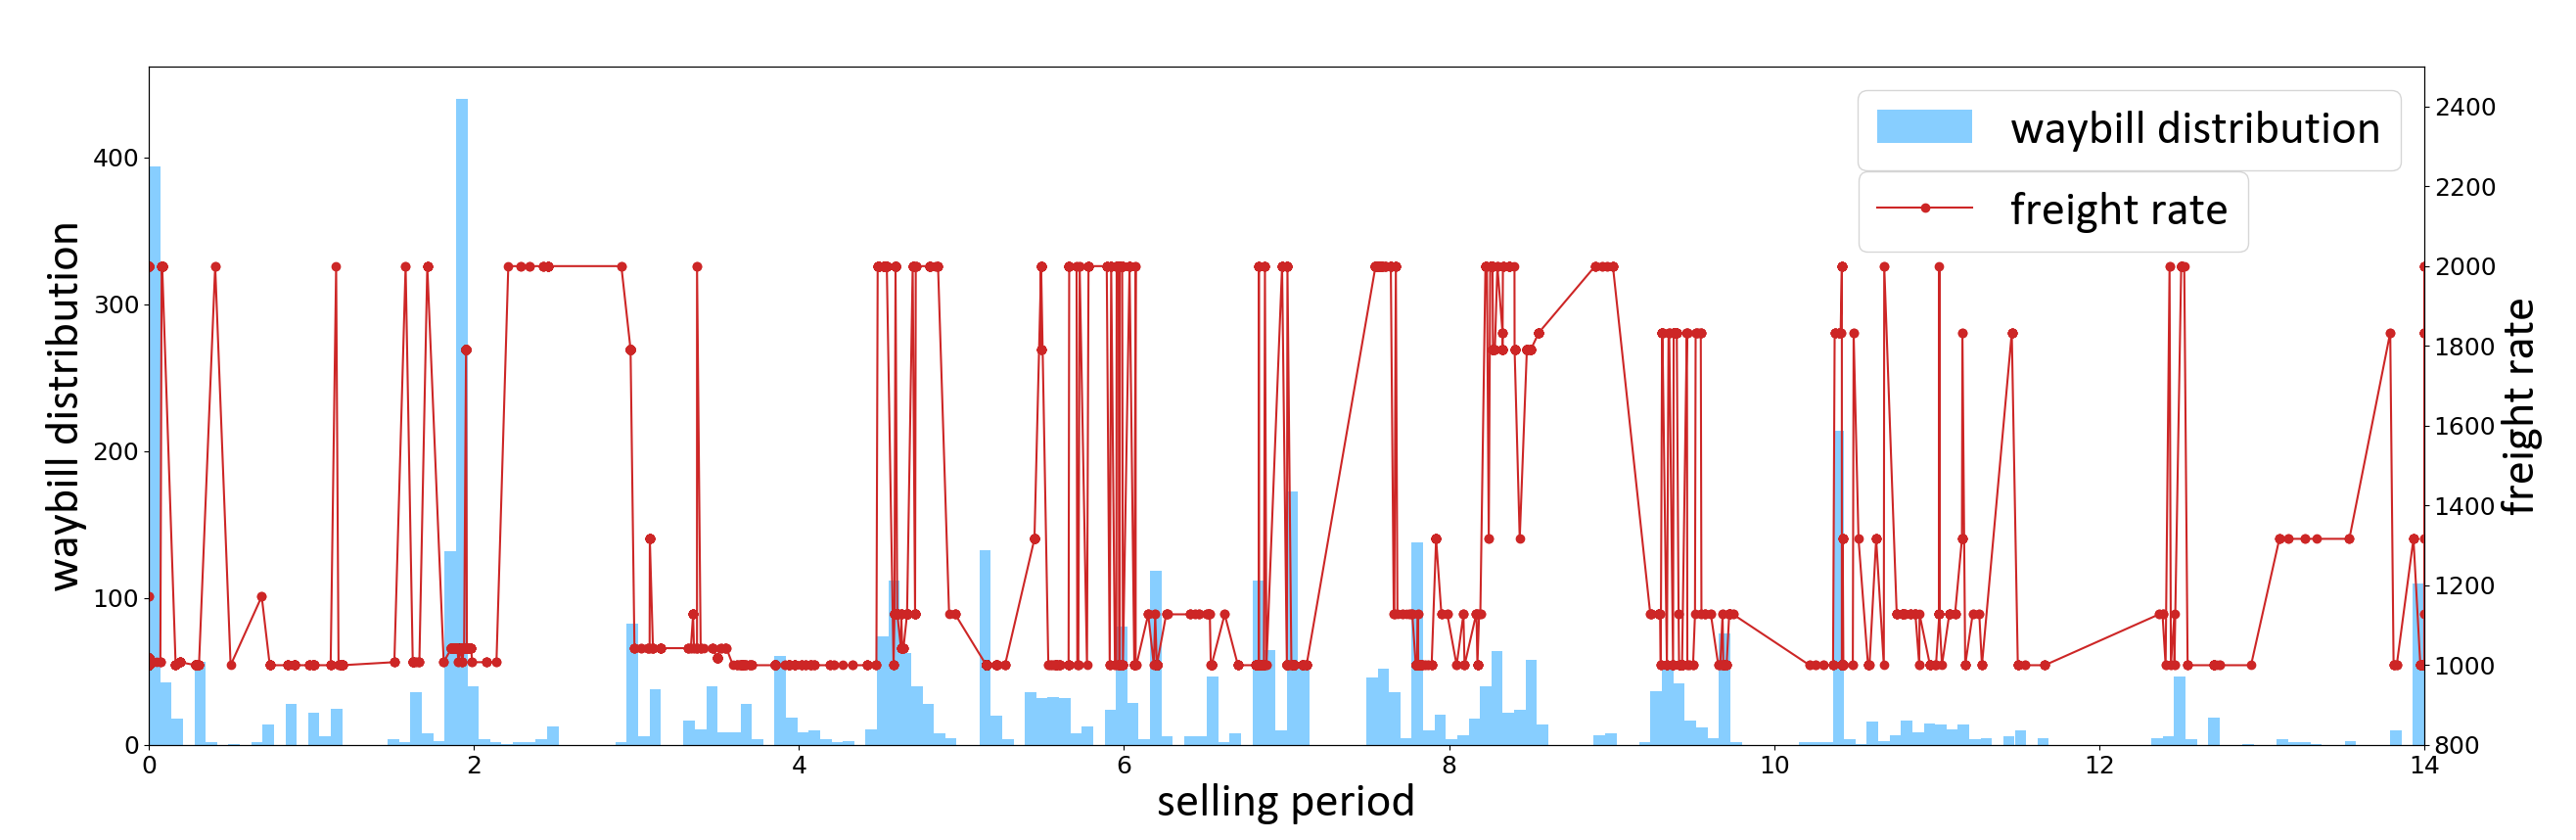
\includegraphics[scale=0.2]{Chapter-Mock/images-Mock/WF-S1.png}
    \label{fig:Mock-The Evolution Trend of Waybill Distribution and Freight Rate}
    }
    \quad
    \subfigure[Partial.]{
    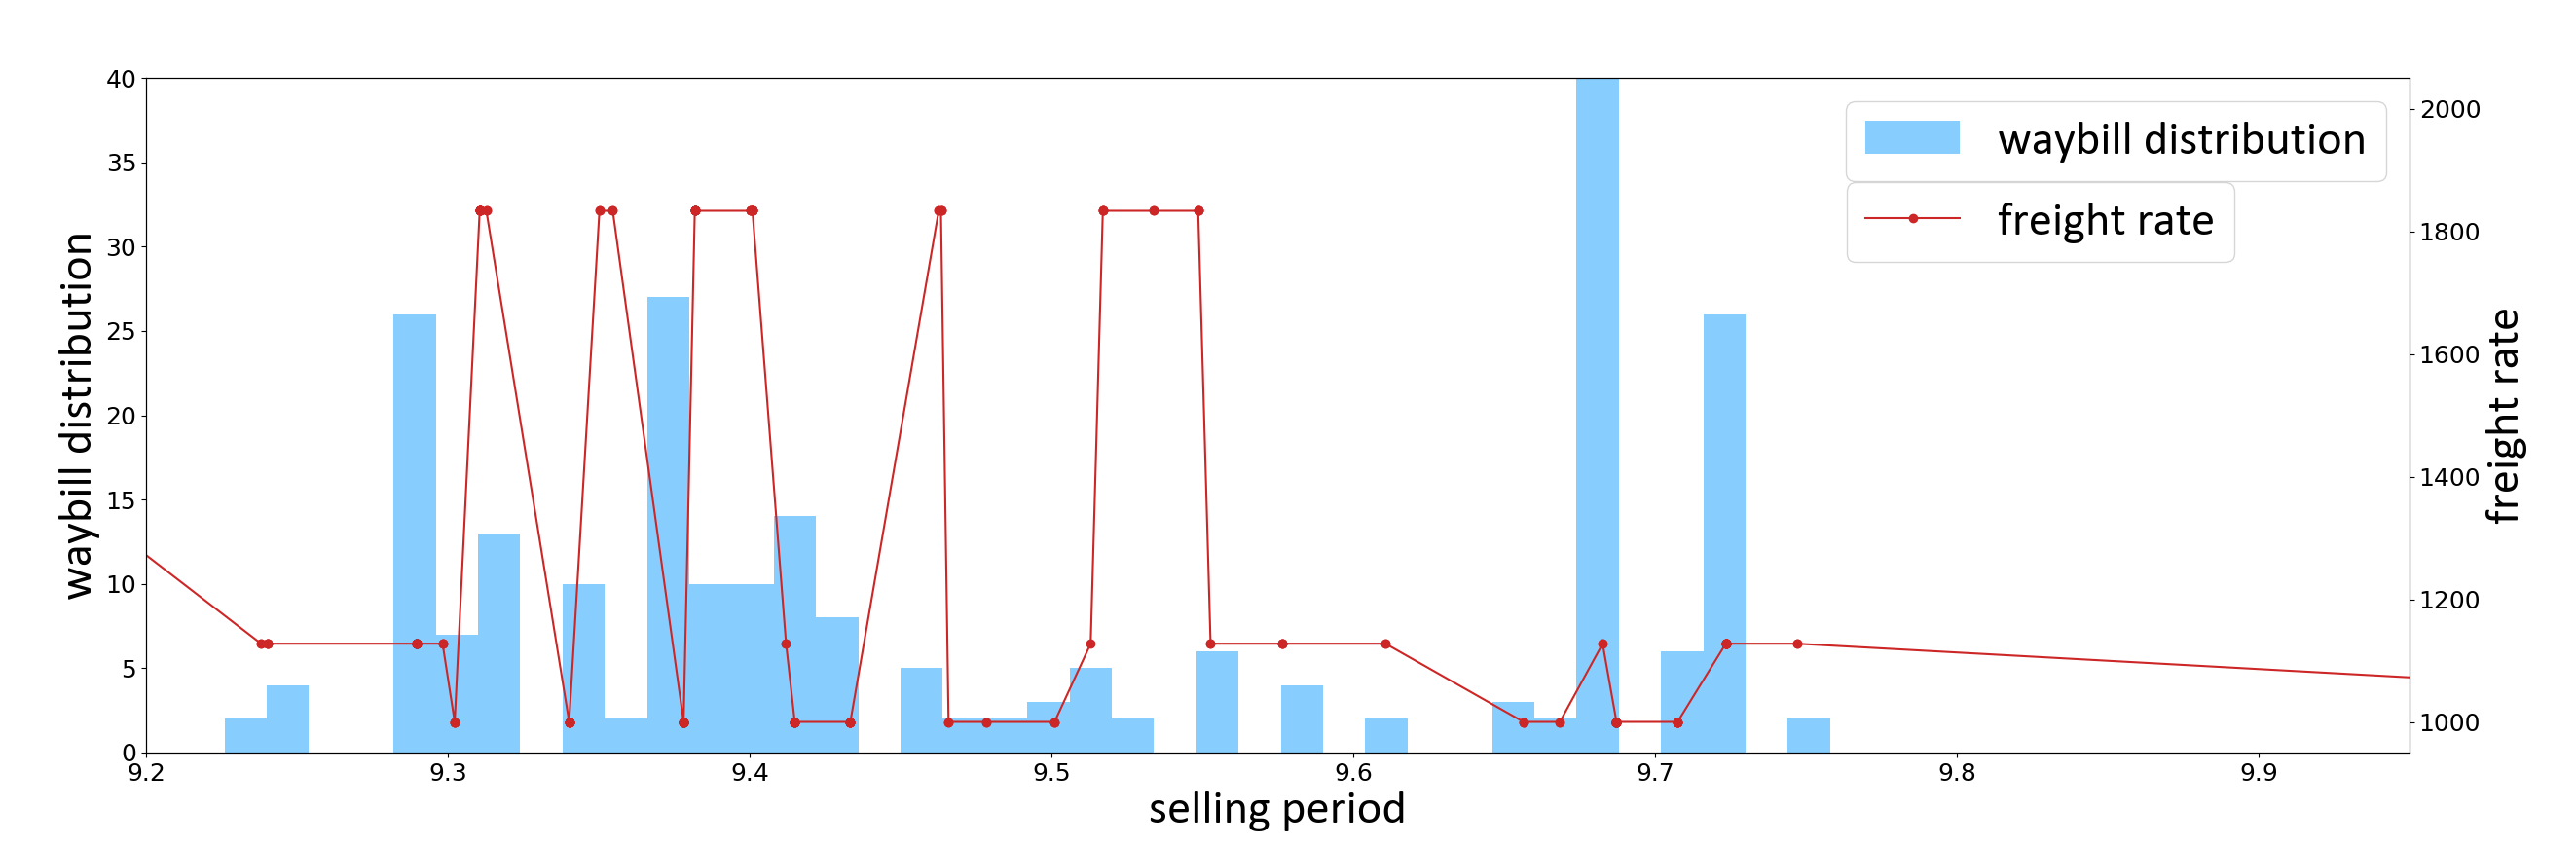
\includegraphics[scale=0.2]{Chapter-Mock/images-Mock/WF-S2.png}
    \label{fig:Mock-The Evolution Trend of Waybill Distribution and Freight Rate-zoom}
    }
    \caption{The Evolution Trend of Waybill Distribution and Freight Rate.}
\end{figure}

It can be concluded from the above research that when the freight is relatively low, customers tend to book containers, and when the freight is high, customers will continue to wait. This behavior indicates that customers are more willing to buy at low prices. These analysis also help us to discover the other relationships in later tasks.

\subsection{Task 2(2). Relationship between Sales Volume and Freight Rate}
\subsubsection{Factors: Booking Habits}
In the previous study, we find that the pattern of customers' booking habits has some relationship \parencite{zym} with the trend of freight rate fluctuation, that is, customers will react to changes in prices and the response has a certain lag. To further dig out which is the lag variable, we apply the \textbf{Granger Cause Test} for causal inference.

Granger Cause Test is a well-known method in Statistics to determine if a particular variable comes after another in the time series and what the lags are. It is a bottom up procedure which assumes the data-generating processes in any time series are independent variables; then the data sets are analyzed to see if they are correlated.
%如何检验要不要详细说明
\begin{table}[H]
    \renewcommand\arraystretch{2}   %%控制行间距
    \centering
    \caption{Granger Causality: Number of lags (no zero) 2}
    \begin{tabular}{cc} 
        \toprule
        \specialrule{0em}{1pt}{1pt}
        ssr based F test & F=2.6948, p=0.0181, df\underline{\hbox to 0.2cm{}}denom=101, df\underline{\hbox to 0.2cm{}}num=6\\
ssr based ch12 test & ch12=18.2498, p=0.0056, df=6\\
likelihood ratio test & ch12=16.9283, p=0.0096, df=6\\
        \specialrule{0em}{1pt}{1pt}
        \bottomrule
    \label{tbl:Mock-Grange Cause Test}
    \end{tabular}
\end{table}
\vspace{-0.8cm}
From the results in Table \ref{tbl:Mock-Grange Cause Test}, we can claim with at least 95 percent confidence level that the order number comes after the freight rate and the lags are 6 data points. As we have divided the 14-day selling period into 120 time slices, this results means that plenty waybill orders often come after decrease in freight rate with lags within 17 hours.%是不是要继续探寻其他流向的反应时间

So far, we can get the conclusion that, on a small time scale, changes in freight rates will greatly affect customer booking behavior and further affect sales volume.The specific manifestation is that when the freight rate increases compared with the previous period, sales will decrease; when the freight rate decreases compared with the previous period, the sales increase, but there is a certain amount of lag in the reaction process.
\subsubsection{Factors: Market Demand}
In addition, we also consider the impact of changes in the macro market on sales and pricing. We \textbf{assume that the demand generated by the market must be realized within the next 14 days}, that is, the customers in need must make the predetermined behavior within the next 14 days. The reason why we choose the 14-day period is that the usual shipping period is 14 days, which not only fully considers the waiting time for customers to order, but also simplifies our model. And the sales period is divided into 14 days.

Here we define the symbol of the market demand index as $M$, and the market demand index on the i\^th day as $M_i$, where $i\in\{0,1,\dots,n \}$. This results in a set of market demand for each day of the sales period. We denote this set by：$$[M_0\quad M_2\quad \dots \quad M_{n}]$$

According to the analysis in task2.(1), we can get the percentage of sales order distribution during the same flow up sales period. Then we define the set by:
$$[a_0\quad a_2\quad \dots \quad a_{13}], subject\quad to \sum_{i=0}^{13}a_i = 1.$$

And we define the sales volume on the i\^th day as $T_j$, where $j\in\{1,2,\dots,n+13 \}$ and  $T_j = 0$, when $j < 14$.
Then there is the following equation：
\begin{equation}
{
    \begin{bmatrix}
        T_{1} & T_{2} & \cdots & T_{14} \\
        T_{2} & \ddots &        & \vdots\\
        \vdots &       & \ddots  &\vdots  \\
        T_{n} & \cdots &\cdots & T_{n+13}
    \end{bmatrix}
}
\times
{\left[
    \begin{array}{cc}
         a_0  \\
         a_1  \\
         \vdots\\
         a_{13}
    \end{array}
\right ]}
=
{\left[
    \begin{array}{cc}
         M_{0}  \\
         M_{1}  \\
         \vdots\\
         M_{n-1}
    \end{array}
\right ]}
\label{eq:Cal market index}
\end{equation}\\
\vspace{-0.1cm}
Next, we can solve $M_0\sim M_{n-1}$ based on the known sales volume data. This means that we can get the history market demand index according to the current sales volume. Then we can use the above algorithm to dig out the market demand index of each flow direction from the data set and show its fluctuation trend over time. We choose three flow directions Yingkou-Ningbo, Xingang-Nansha and Yingkou-Nansha to show in Fig.\ref{Fig:a}.

\begin{figure}[H]
    \centering
    \subfigure[Yingkou-Ningbo.]{
    \begin{minipage}[t]{\linewidth}
    \centering
    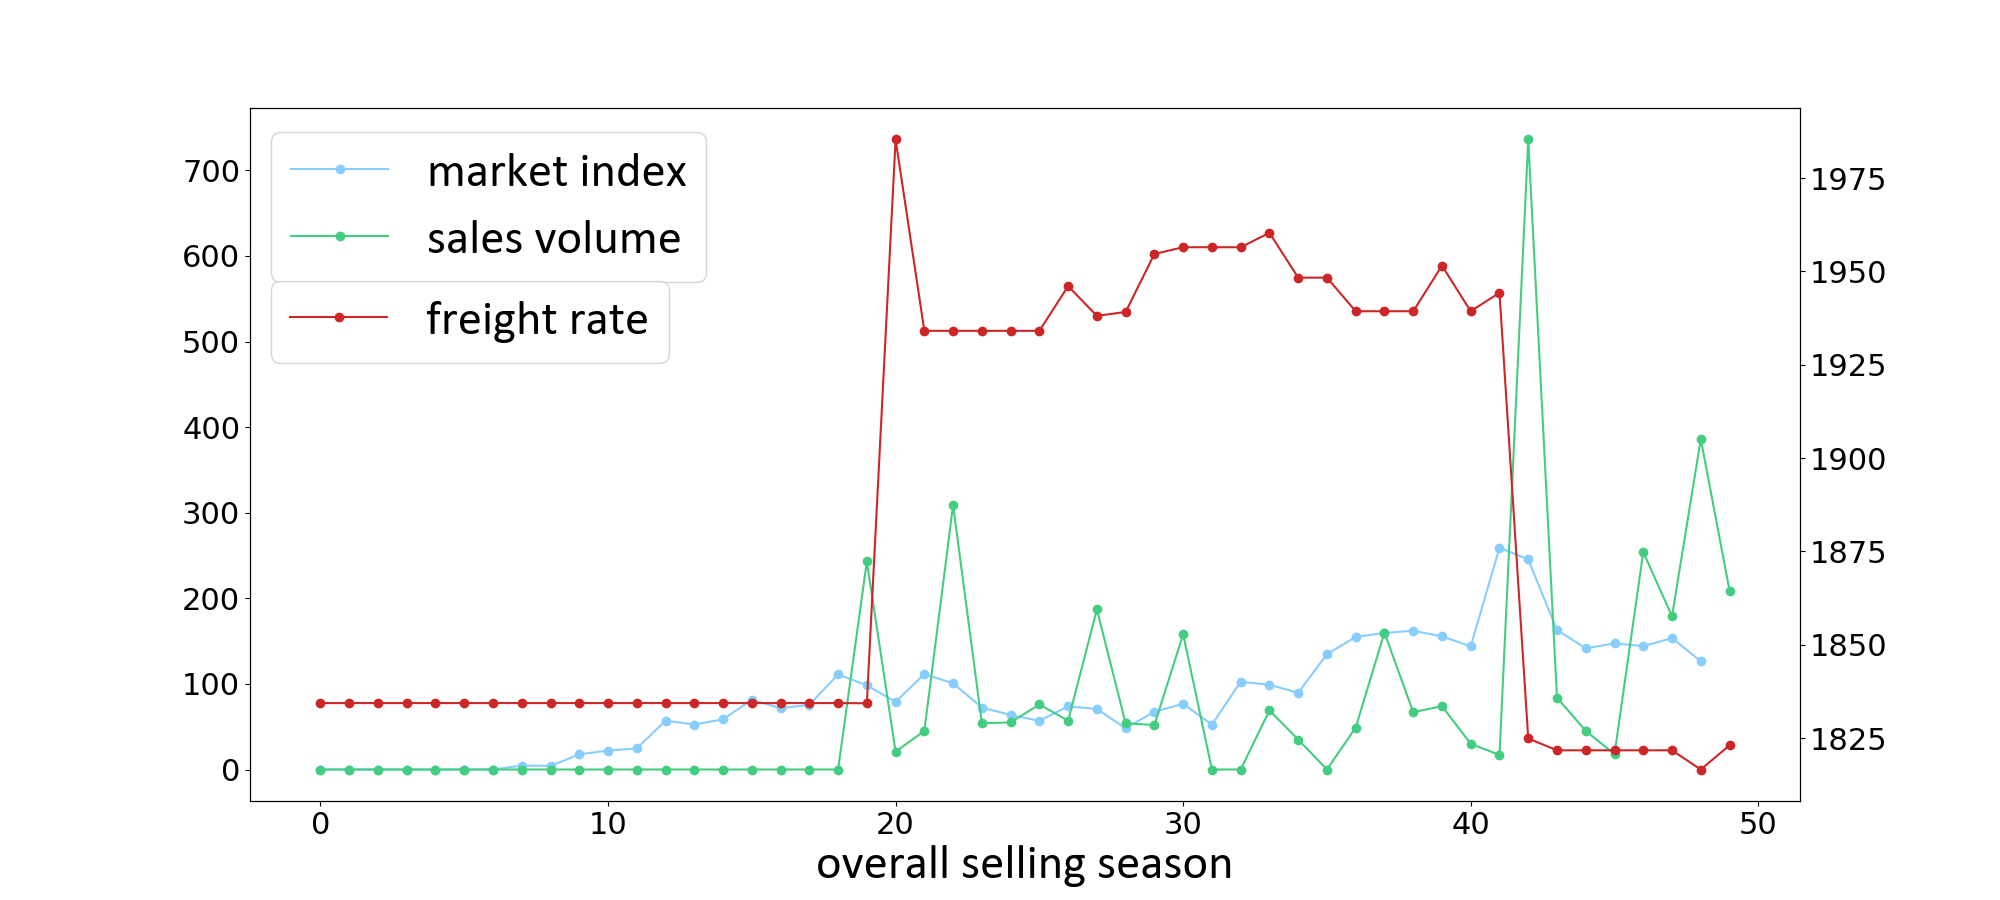
\includegraphics[scale = 0.3]{Chapter-Mock/images-Mock/2_2_1.png}
    \end{minipage}
    }\\
    \subfigure[Xingang-Nansha.]{
    \begin{minipage}[t]{\linewidth}
    \centering
    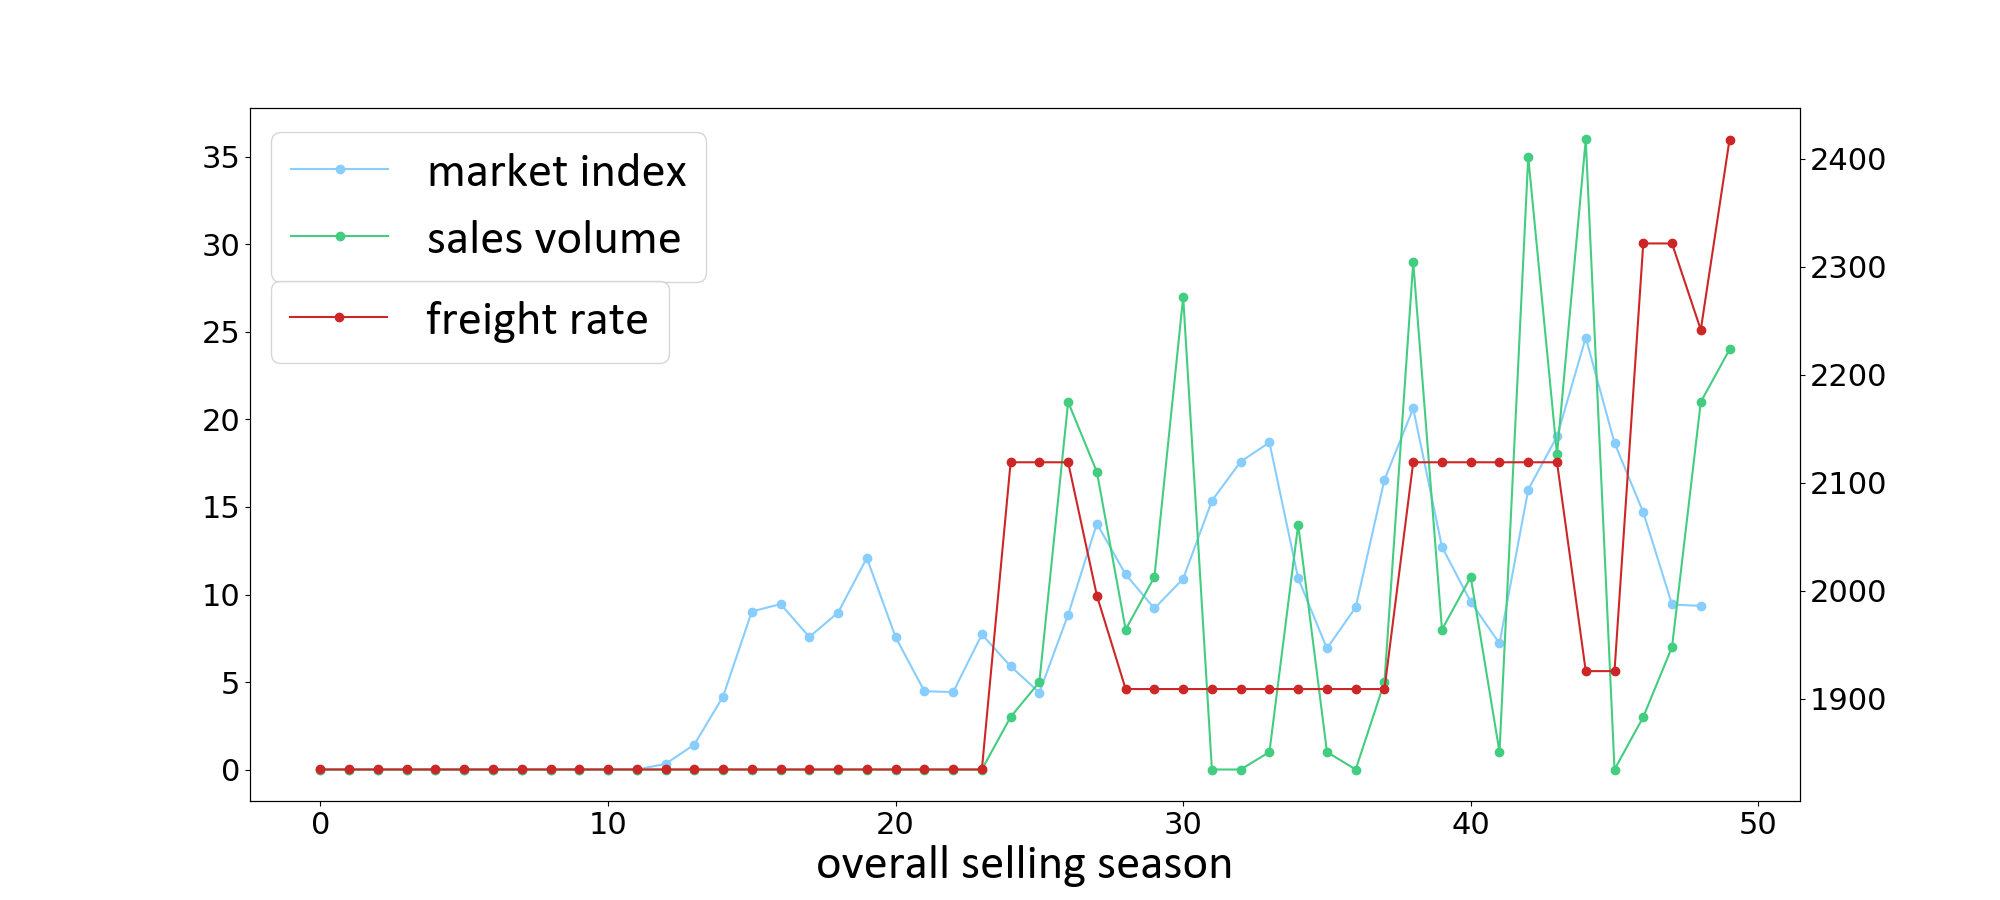
\includegraphics[scale = 0.3]{Chapter-Mock/images-Mock/2_2_2.png}
    \end{minipage}
    }\\
    \subfigure[Yingkou-Nansha.]{
    \begin{minipage}[t]{\linewidth}
    \centering
    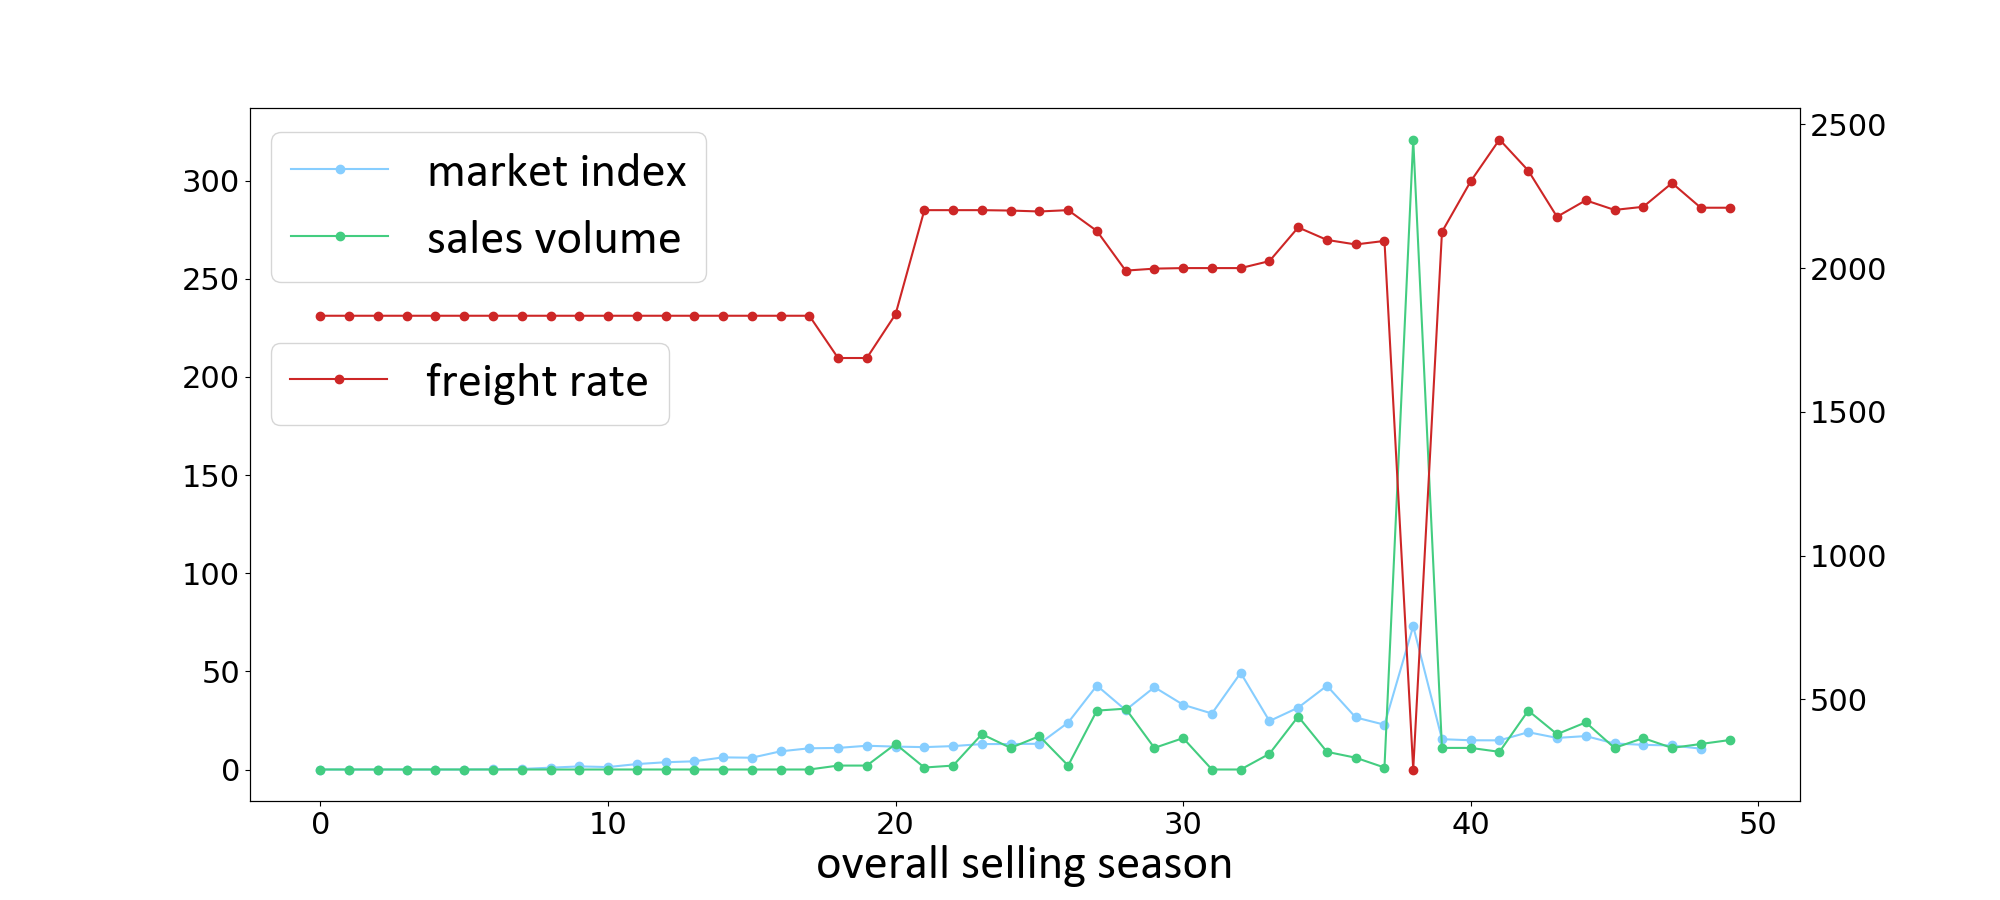
\includegraphics[scale = 0.3]{Chapter-Mock/images-Mock/2_2_3.png}
    \end{minipage}
    }
    \caption{Market demand index fluctuation.}
    \label{Fig:a}
\end{figure}

According to the definition we have made, the market demand index will imply the future sales volume, which means that the correlation between sales volume and market demand is positive. Combined with the changing curve of the freight rate, we find that when the sales volume rises, the freight rate will decrease, and vice versa. There is a negative correlation between the two. Furthermore, we can get such a relationship: the shipping market demand index will positively affect the future sales of containers, and the freight rate will be adjusted according to the sales.

To sum up, we can summarize the relationship between sales volume and freight rate as follows: customers will decide the transaction time due to the freight rate, which is reflected in the sales distribution in a certain selling period; the market demand will affect the future sales volume, and the freight rate will be adjusted  based on sales volume. In short, the freight rate will affect the sales volume, and the sales volume will also influence the freight rate.

\subsection{Task 2(3). Prediction of Market conditions}
In the above analysis, we obtain the value of the market demand index and get its volatility curve over time. From this analysis, we grasp the influence of changes in market demand on sales, which is conducive to the pricing of freight rates. Therefore, a short-term forecast of market conditions is very beneficial to the design of the next pricing system.

In this regard, we tend to reflect future market trends by forecasting sales volume. We use Long and Short-Term Memory (LSTM)  to make a prediction of sales volume based on existing time series data\parencite{2016LSTM}.

LSTM model  is a variant of recurrent neural network (RNN). It is well-suited to classifying, processing and making predictions based on time series data. A common LSTM unit is composed of a cell, an input gate, an output gate and a forget gate. The cell remembers values over arbitrary time intervals and the three gates regulate the flow of information into and out of the cell\parencite{lstm1}.

Some specific applying details of the model:

\begin{enumerate}[\quad\bf1.]
\item Input and Output

We first group the market demand index sequence three at a time to construct a training matrix, and then label each of them with the exact index coming right after them. Therefor, our input of the model is a 3-dimension index sequence and the output of the model is one predicted index. 
\item Loss Function

During the training, we use mean square error (MSE) as the loss function:
\begin{equation}
    MSE(x, \hat{x})=\frac{1}{N}\sum_{i=1}^N (x_i-\hat{x_i})^2
\end{equation}

where $x$ is the true target vector and $\hat{x}$ is the predicted feature vector and $N$ is the number of dimension.

\item Training parameters

The number of units of LSTM layer is set to 200 and the whole model contains 482,601 trainable parameters. Our model is trained for 100 epochs with ADAM optimizer.
\end{enumerate}

\begin{table}[H]
    \renewcommand\arraystretch{2}   %%控制行间距
    \centering
    \caption{Prediction model summary}
    \begin{tabular}{ccc}    %%三列均左对齐
        \toprule  %%表格横线加粗
        \specialrule{0em}{2pt}{2pt}    %%添加透明线控制行高
        Layer (Type) & Output Shape & Param \\
        \specialrule{0em}{2pt}{2pt}    %%添加透明线控制行高
        \midrule
        \specialrule{0em}{1pt}{1pt}
        LSTM & (None, 200) & 161600 \\
        Repeated Vector & (None, 1, 200) & 0 \\
        LSTM & (None, 1, 200) & 320800 \\
        Time Distributed & (None, 1, 1) & 201 \\
        \specialrule{0em}{1pt}{1pt}
        \bottomrule
    \label{tbl:Mock-LSTM summary.}
    \end{tabular}
\end{table}
\vspace{-0.8cm}

We select partial sequence from three flow directions to make short-term forecasts and compare the results with raw data. With the predicted market demand index, we can compute the future sales volume using formula \ref{eq:Cal market index}.

\begin{figure}[H]
    \centering
    \subfigure[Yingkou-Ningbo.]{
    \begin{minipage}[t]{0.3\linewidth}
    \centering
    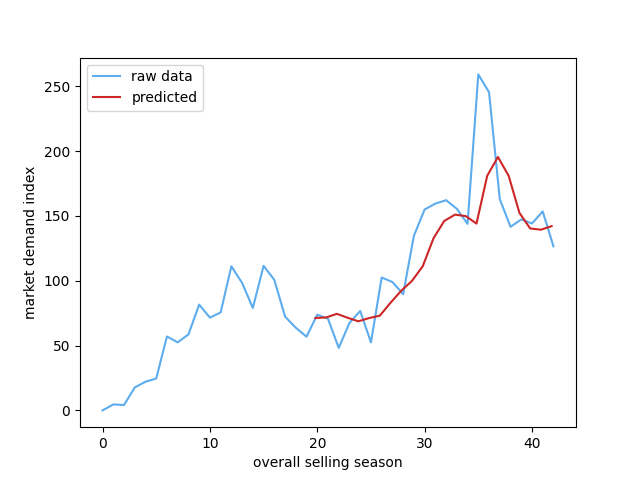
\includegraphics[scale = 0.3]{Chapter-Mock/images-Mock/LSTM_market.png}
    \end{minipage}
    }
    \subfigure[Xingang-Nansha.]{
    \begin{minipage}[t]{0.3\linewidth}
    \centering
    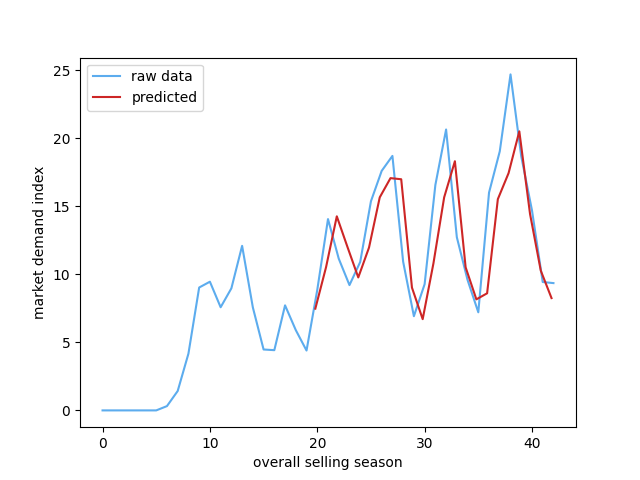
\includegraphics[scale = 0.3]{Chapter-Mock/images-Mock/LSTM_market_2.png}
    \end{minipage}
    }
    \subfigure[Yingkou-Nansha.]{
    \begin{minipage}[t]{0.3\linewidth}
    \centering
    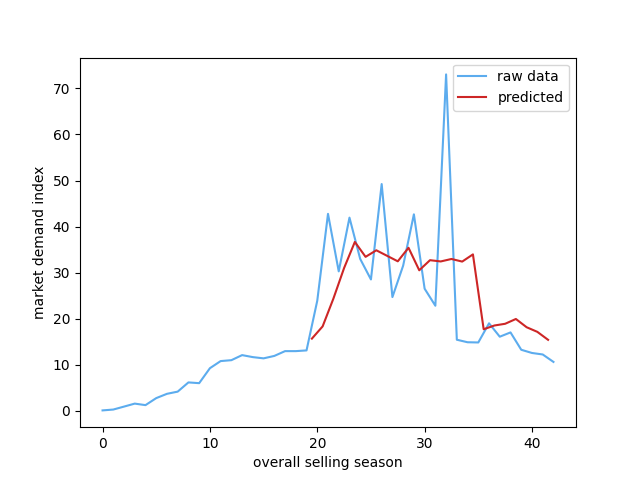
\includegraphics[scale = 0.3]{Chapter-Mock/images-Mock/LSTM_market_3.png}
    \end{minipage}
    }
    \caption{Short-term forecasts of Market Demand Index using LSTM}
    \label{Fig:Short-term of Sales Volume using LSTM}
\end{figure}


\begin{figure}[H]
    \centering
    \subfigure[Yingkou-Ningbo.]{
    \begin{minipage}[t]{0.3\linewidth}
    \centering
    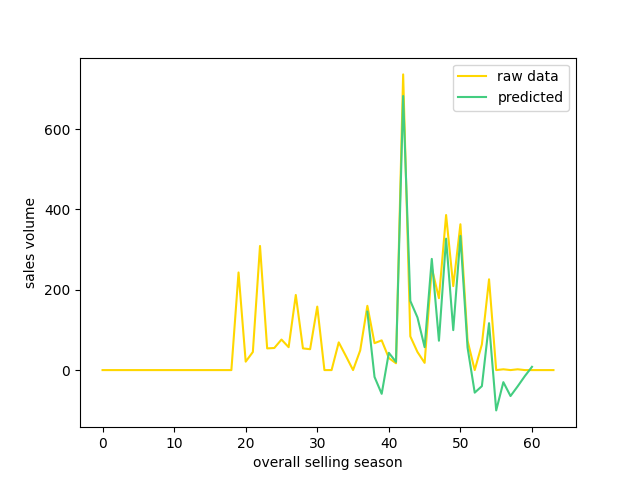
\includegraphics[scale = 0.3]{Chapter-Mock/images-Mock/LSTM_sale.png}
    \end{minipage}
    }
    \subfigure[Xingang-Nansha.]{
    \begin{minipage}[t]{0.3\linewidth}
    \centering
    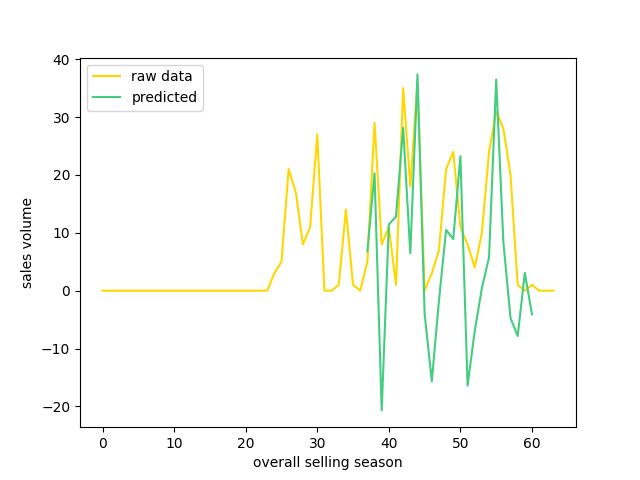
\includegraphics[scale = 0.3]{Chapter-Mock/images-Mock/LSTM_sale_2.png}
    \end{minipage}
    }
    \subfigure[Yingkou-Nansha.]{
    \begin{minipage}[t]{0.3\linewidth}
    \centering
    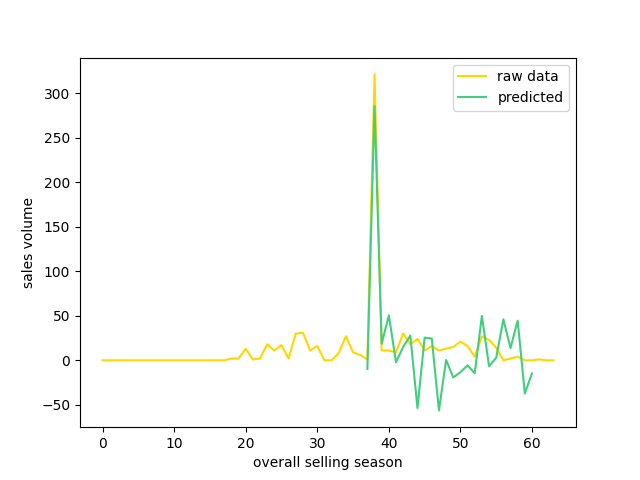
\includegraphics[scale = 0.3]{Chapter-Mock/images-Mock/LSTM_sale_3.png}
    \end{minipage}
    }
    \caption{Sales volume calculated by prediction}
    \label{Fig:Sales volume calculated by prediction}
\end{figure}

As shown in Fig. \ref{Fig:Short-term of Sales Volume using LSTM}, the market demand of Yingkou-Ningbo and Yingkou-Nansha will meet a small peak according to raw data and is correctly predicted by our model. As for Xingang-Nansha, our model have predicted exact the same fluctuation with raw data. In Fig. \ref{Fig:Sales volume calculated by prediction}, the sales volume caculated by our prediction matches raw data well, which means that our model is reasonable for the prediction of sales volume and can be further applied in the following study. 




